
\section{Optimal Control for SHE}

Since the SHE problem is equivalent to controlling a dynamic system from the origin of coordinates to a specific point, we must formulate a control problem that solves this task but also complies with the restrictions on the values that the control can take. It is necessary to set a finite subset $ \mathcal {U} $ of the interval $ [- 1,1] $, the optimal control is such that it can only take the values allowed in the discretization. In other words, the control problem is:

\begin{problem}[OCP for SHE]\label{OCP1}
    Given two sets of odd numbers $ \mathcal {E} _a $ and $ \mathcal {E} _b $ and given the target vector $ \bm {x} _T \in \mathbb {R} ^ {N_a + N_b} $, also given a set $ \mathcal {U} $ of admissible controls, we look for the function $ u (\tau) \ | \ \tau \in [0, \pi) $ such that:
    %
    \begin{gather}
        \min_{u(\tau) \in \mathcal{U}}         
         \Bigg[ \frac{1}{2}|| \bm{x}(\pi) - \bm{x}_T  ||^2 \Bigg]  \\
        \notag \text{suject to: } \\
        \begin{cases}
            \dot{\bm{x}}(\tau) = \bm{\mathcal{D}}(\tau) u(\tau)  & \tau \in [0,\pi)\\
            \bm{x}(0) = {0}
        \end{cases}
    \end{gather}
\end{problem}
%
The solution of this control problem is complex due to the restriction on the admissible control values.
%
In order to obtain a problem that can be solved by classical control theory we can formulate the following control problem:

\begin{problem}[Regularized OCP for SHE]\label{OCP1}
    Given two sets of odd numbers $ \mathcal {E} _a $ and $ \mathcal {E} _b $ and given the target vector $ \bm {x} _T \in \mathbb {R} ^ {N_a + N_b} $, we look for the function $ |u (\tau)|<1 \ | \ \tau \in [0, \pi) $ such that:

    \begin{gather}
        \min_{|u(\tau) |<1}         
         \Bigg[ \frac{1}{2}|| \bm{x}(\pi) - \bm{x}_T  ||^2  
        + \epsilon \int_0^{\pi} \mathcal{L}(u(\tau)) d\tau \Bigg]  \\
        \notag \text{suject to: } \\
        \begin{cases}
            \dot{\bm{x}}(\tau) = \bm{\mathcal{D}}(\tau) u(\tau)  & \tau \in [0,\pi)\\
            \bm{x}(0) = {0}
        \end{cases}
    \end{gather}
\end{problem}

Where we will choose $ \mathcal {L}: \mathbb {R} \rightarrow \mathbb {R} $ such that the optimal control $ u^* $ only takes values in the discretization $ \mathcal {U} $ of the interval $ [- 1.1] $. Furthermore, the parameter $ \epsilon $ should be small so that the solution minimizes the distance from the final state and the target.
%
Next we will study the optimality conditions of the problem, for a general $ \mathcal {L} $ function, and then specify how $ \mathcal {L} $ should be so that the optimal control $ u ^ * $ only takes the allowed values in $ \mathcal {U} $.

\subsection{Optimality conditions}

To write the optimility conditions of the problem we will use the principle of the Pontryagin minimum. For them it is necessary to define the Hamiltonian of the system, which in this case is:
\begin{gather}\label{hamil}
    H(u,\bm{p},\tau) = 
    \epsilon \mathcal{L}(u) + 
    [\bm{p}^T(\tau) \cdot \bm{\mathcal{D}}(\tau)]
    u(\tau)
\end{gather}

Where the variable $ \bm{p} (\tau) $ called attached state is introduced, which is associated with the restriction imposed by the system. From the Hamiltonian, the following optimality conditions can be written:
\begin{enumerate}

    \item \textbf{Final condition of the adjoint}: This optimiality condition is obtained from the final cost of the control problem in this case $ \Psi (\bm{x}) = \frac {1}{2} \| \bm{x} (\pi) - \bm{x}_T \|^2 $.
    \begin{gather}
        \bm{p}(\pi) = \nabla_{\bm{x}} \Psi(\bm{x}) =  (\bm{x} (\pi) - \bm{x}_T)
    \end{gather}
    \item \textbf{Adjoint evolution equation}:
    \begin{gather}
        \dot{\bm{p}}(\tau) = -\nabla_x H(u(\tau),\bm{p}(\tau),\tau) = 0
    \end{gather}
    From where it can be deduced that $ \bm {p} (\tau) = \text {cte} $ so that $ \bm {p} (\tau) = \bm {x} (\pi) - \bm { x} _T \ | \ \forall \tau \in [0, \pi) $ so from now on we will refer to it simply as $ \bm {p} $, noting that it is invariant in time.
    \item \textbf{Optimal control shape}: We known that $ u^* = \argmin_{|u|<1} H(\tau,\bm{p}^*,u)$, so in this case we can write:
    \begin{gather}
        u^*(\tau) = \argmin_{|u|<1}  \Big[   \epsilon \mathcal{L}(u(\tau)) + 
        [{\bm{p}^*}^T \cdot \bm{\mathcal{D}}(\tau)]
        u(\tau) \Big]
    \end{gather}
    Therefore, this optimality condition reduces to the optimization of a function in a variable within the interval $ [- 1,1] $. We need note that the value of $[{\bm{p}^*}^T \cdot \bm{\mathcal{D}}(\tau)]$ is unknow but we know that this value can change the sign. So we need design the $\mathcal{L}$ to the optimal control $u^*$ must be a some element of $\mathcal{U}$ for every value of $[{\bm{p}^*}^T \cdot \bm{\mathcal{D}}(\tau)]$. For this study, we build a function $H^*: [-1,1] \rightarrow \mathbb{R}$ such that:
    \begin{gather}
        H^*(u) = \epsilon \mathcal{L}(u) + mu  |  \forall m \in \mathbb{R}
    \end{gather}
    If we found a function $\mathcal{L}$ such that its minimums in interval $[-1,1]$ are in $\mathcal{U}$ the solutions of regularized optimal control are in $\mathcal{U}$.
\end{enumerate}
%
\subsection{Conditions for bi-level and tri-level controls}
%
Since we need the optimal control $ u ^ * $ to be \emph {bang-bang}, we must design $ H ^ * (u) $ so that its minimum is at the extremes of the interval $ [- 1,1] $ .
%
In the case of a variable (this case) we can only achieve this behavior if there is no minimum within the interval.
%
One way to ensure this behavior is to take the function $ H ^ * (u) $ concave, by choosing the term $ \mathcal {L} (u) $.
%
This is because the concavity of the term $ \mathcal {L} (u) $ determines the concavity of the Hamiltonian $ H ^ * (u) $ thanks to the fact that the second derivative of $ H ^ * (u) $ is proportional to the second derivative of the penalty term, that is:
\begin{gather}
    \frac{d^2{H^*}}{du^2} = \epsilon \frac{d^2\mathcal{L}}{du^2} 
\end{gather}

In this way whenever we choose a penalty term such that:

\begin{gather}
    \frac{d^2\mathcal{L}}{du^2} \leq 0 
\end{gather}

we will obtain a concave $ H ^ * (u) $ function within a convex interval giving rise to an optimal control $ u ^ * $ \ emph {bang-bang}. We can see an illustration of this behavior in the figure (\ref {bang-bang}).
\newline

\begin{figure}[!ht]
    \centering
    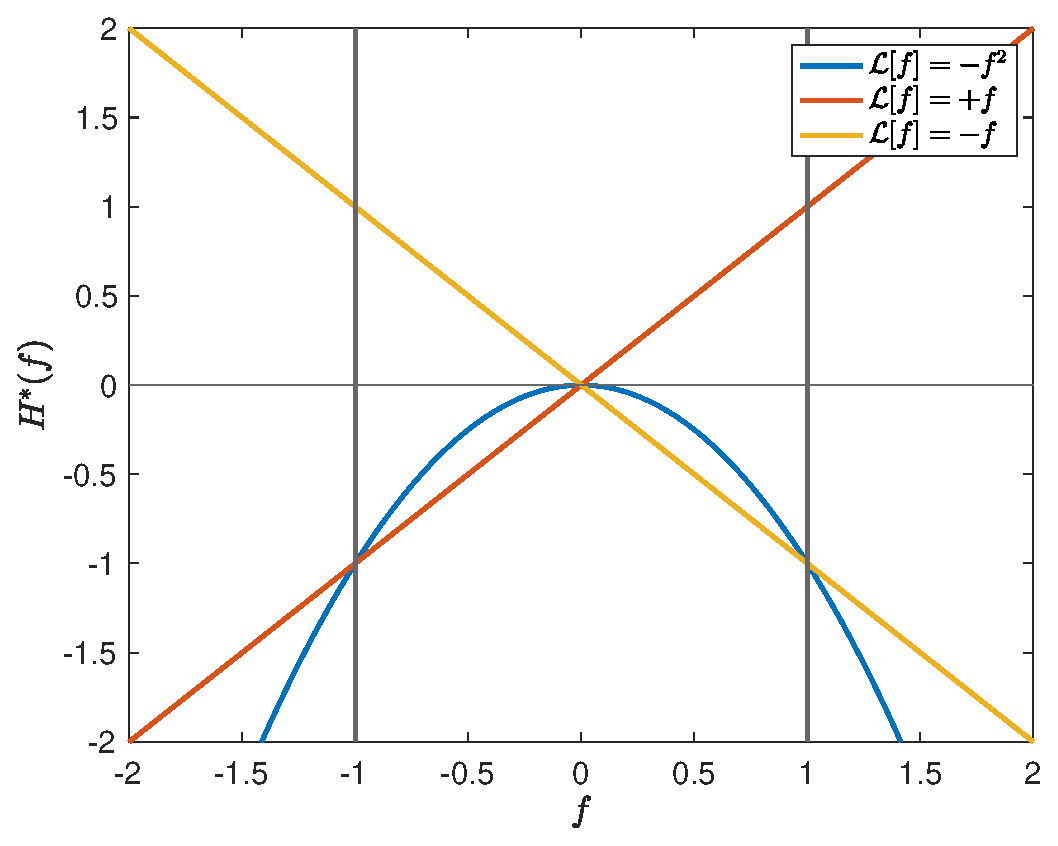
\includegraphics[scale=0.5]{img/bang-bang.eps}
    \caption{Ilustración sobre el comportamiento de la función $H^*(u)$ para distintos términos de penalización $\mathcal{L}(u)$. El problema de minimización de $H^*(u)$ con respecto a $f$ para las distintas curvas presentadas en la figura siempre tiene minimos en los extremos del intervalo $[-1,1]$ de manera que el control óptimo en los tres casos, será \emph{bang-bang}.}
    \label{bang-bang}
\end{figure}

\subsection{Condiciones  para la obtención de controles multi-nivel}

Dado que necestiamos que existan mínimos de la función $H^*(u)$ en el interior del intervalo $[-1,1]$ la función $\mathcal{L}$ no podrá ser convexa. Además si queremos que los minimimos para cualquier valor de $m \in \mathbb{R}$ solo tome valores finitos esta función de ser no diferenciable. De manera que un variación infinitesimal de $m$ mantenga constante el mínimo de $\mathcal{L}(u)$. Proponemos una función $\mathcal{L}$ como una aproximación afin tomando como vértices los puntos pertenecientes al conjunto $\mathcal{U}$.
